\addtocontents{toc}{\protect\newpage}
\section{Empirical Study}\label{sec:empirical-study}

In this section, we demonstrate the effectiveness of machine learning for trade classification in an empirical setting. To commence, the construction of datasets is presented.

\subsection{Data and Data Preparation}\label{sec:data-and-data-preparation}

% \todo{This paper employs one of the largest data sets in recent intraday options literature.}
The following chapter describes the construction of datasets, that suffice the data requirements of classical trade classification rules and for our machine learning models. We also discuss how we define and infer the true trade initiator.

\subsubsection{Data Collection}\label{sec:data-collection}

% \textbf{Data Sources}

Testing the empirical accuracy of our approaches requires option trades where the true initiator is known. To arrive at a labelled sample, we combine data from four individual data sources. Our primary source is LiveVol, which records option trades executed at US option exchanges at a transaction level. We limit our focus to option trades executed at the \gls{CBOE} and \gls{ISE}. LiveVol contains both trade and matching quote data. Like most proprietary data sources, it does not distinguish the initiator nor does it include the involved trader types. For the \gls{CBOE} and \gls{ISE} exchange, the \gls{ISE} Open/Close Trade Profile and \gls{CBOE} Open-Close Volume Summary contain the buy and sell volumes for the option series by trader type aggregated on a daily level. A combination of the LiveVol dataset with the open/close data, allows us to infer the trade initiator for a subset of trades. For evaluation and use in some of our machine learning models, we acquire additional underlying and option characteristics from IvyDB's OptionMetrics.

% \textbf{Trade Initiator}

In \cref{sec:trade-initiator} we discussed three views on the trade initiator. As our data sources do not provide the order entry times or order types for both sides of the trade, we define the trade initiator based on the position relative to the market maker, who caters to the liquidity demand. More specifically, we classify customer trades as buyer-initiated if the trade is due to a customer buy order and as seller-initiated for customer sales. As previous literature, e.g., \textcite[][4276]{garleanuDemandBasedOptionPricing2009} suggests that trader types, for example, proprietary traders, have a similar role to market makers by supplying liquidity, we limit our analysis to trades between customers and market makers for which the picture is unambiguous. Our definition is consistent with the of \textcite[][8]{grauerOptionTradeClassification2022}.

% \textbf{Sample Construction}

Our sample construction follows \textcite[][7--9]{grauerOptionTradeClassification2022}, fostering comparability between both works. We acquire transaction-level options trade data for all major US exchanges from LiveVol. The dataset is tabular, and each record is time-stamped to the second. For each transaction, the executing exchange, trade price, trade volume, quotes and quote sizes for the exchanges where the option is quoted, as well as the \gls{NBBO} are recorded. This is sufficient to estimate the quote rule, depth rule, and trade size rule. In addition, for tick-based algorithms, we add the previous and subsequent distinguishable trade prices. We can uniquely identify the traded option series from a distinct key consisting of the underlying, expiration date, option type and strike price. Our analysis is conducted on transactions at the \gls{ISE} and \gls{CBOE}. To purge the data of potential errors, we filter out:
\begin{enumerate}[label=(\roman*),noitemsep]
    \item trades with a trade price $\leq 0$,
    \item trades with a trade volume $\leq 0$ or $\ge \num{10000000}$ contracts,
    \item cancelled or duplicated trades,
    \item entries with multiple underlying symbols for the same root.
\end{enumerate}

The open/close datasets for the \gls{ISE} and \gls{CBOE} contain the daily buy and sell volumes for the option series by trader type, the trade volume and whether a position was closed or opened. Four trader types are available: customer, professional customer, broker/dealer, and firm proprietary. Customer orders are placed by a retail trader or a member of the exchange on behalf of the customer. Professional customers are distinguished from the former by a high trading activity ($\geq390$ orders per day over one month period). Likewise, trades by a member are classified as proprietary, if executed for their account or broker/dealer if placed for non-members of the exchange \autocite[][2]{nasdaqincFrequentlyAskedQuestions2017}. Trades of customers and professional customers are detailed by trade volume ($\leq 100$; 101--199; $> 199$ contracts). As well as, if a position is newly opened or closed. We first sum buy and sell orders of all trader types and volumes to obtain the daily trading volumes at the \gls{ISE} or \gls{CBOE} per option series and day. Separately for the customer buy and sell volumes, we calculate the daily aggregates identified by the account type customer.

To infer the true label, we exploit that, if there were only customer buy or sell orders, hence the customer buy or sell volume equals the daily trading volume, we can confidently sign all transactions for the option series at the specific date and exchange as either buyer- or seller-initiated. Our labelling approach fails in the presence of non-customer or simultaneous customer buy or sell trades. The so-obtained trade initiator is merged with the LiveVol trades of the exchange based on the unique key for the option series.

For the \gls{ISE} trades, our matched sample spans from 2 May 2005 to 31 May 2017 and includes \num{49203747} trades. The period covers the full history of \gls{ISE} open/close data up to the last date the dataset was available to us. Our matched \gls{CBOE} sample consists of \num{37155412} trades between 1 January 2011 and 31 October 2017. The sample period is governed by a paradigm shift in the construction of the \gls{CBOE} open/close dataset and the most recent trade in our LiveVol subscription.

Following our initial rationale for using semi-supervised methods, we reserve unlabelled trades between 24 October 2012 and 24 October 2013 at the \gls{ISE} for pre- and self-training. We provide further details in \cref{sec:train-test-split}. Since LiveVol doesn't distinguish by trader types, this dataset includes both customer and non-customer trades, as well as simultaneous buy and sell trades on the same day.

While our procedure makes the inference of the true trade initiator partly feasible, concerns regarding a selection bias due to the excessive filtering have to be raised. We address these concerns and report summary statistics for unmerged and merged sub-samples in \cref{app:summary-statistics}.

In the following chapter, we motivate feature engineering, present our feature sets and discuss strategies for transforming features into a form that accelerates and advances the training of our models.

\todo{Minor importance of cust-cust trades? “Second, market-makers stand on the liquidity-providing side of most trades. In the options market, market-makers transfer liquidity not only over time but also across different options. With several hundred option contracts available for each underlying, two investors rarely select the same option and thus they are likely to trade with a market-maker. Also, exchange rules grant lead market-makers substantial competitive edge over other liquidity providers (e.g., the 60/40 NBBO order split rule). These rules further strengthen lead market-makers position as the main liquidity providers and make it hard for new players to enter” Found in \textcite{muravyevOrderFlowExpected2016}}

\subsubsection{Data Preprocessing}\label{sec:data-preprocessing}

Classical algorithms infer the initiator of the trade from the \emph{raw} price and quote data. We employ feature engineering to pre-process input data and enhance the convergence and performance of our machine-learning models. Gradient-boosted trees and neural networks, though, flexible estimators have limitations in synthesising new features from existing ones, as demonstrated in empirical work on synthetic data by \textcite[][5--6]{heatonEmpiricalAnalysisFeature2016}. Specifically, ratios, standard deviations, and differences can be difficult for these models to learn and must therefore be engineered beforehand.

\textbf{Features and Feature Sets}

To establish a common ground, we derive three sets of features from raw data. The feature sets, abbreviated as \glsdisp{FS}{FS}, are motivated by features inherent to classical trade classification rules and are consequently derived from quote and price data. Except for a third feature set, which includes additional option characteristics. Distinguished feature sets improve the transferability of our results.

\begin{ThreePartTable}
    \centering
    \begin{TableNotes}\footnotesize
        \item[*] Notation assumes, that the previous or next trade price is distinguishable.
    \end{TableNotes}
    \begin{longtable}{@{}lllllll@{}}


        \caption[Features and Feature Sets]{Features and Feature Sets.}\label{tab:feature-sets}                                                                                                                                                                       \\
        \toprule
        Feature Name            & Definition                                                                                       & Source               & \gls{FS} 1                        & \gls{FS} 2                        & \gls{FS} 3                        \\ \midrule
        \endfirsthead

        \multicolumn{6}{l}{\textit{Continued \tablename~\thetable}}                                                                                                                                                                                                   \\
        \toprule
        Feature Name            & Definition                                                                                       & Source               & \gls{FS} 1                        & \gls{FS} 2                        & \gls{FS} 3                        \\ \midrule
        \endhead

        \bottomrule
        \endfoot

        \insertTableNotes
        \endlastfoot

        trade price             & $P_{i, t}$                                                                                       & tick rule            & \textcolor{viz-green}{\checkmark} & \textcolor{viz-green}{\checkmark} & \textcolor{viz-green}{\checkmark} \\
        price lag (ex)          & $P_{i, t-1}^{\text{ex}}$\tnote{*}                                                                & tick rule            & \textcolor{viz-green}{\checkmark} & \textcolor{viz-green}{\checkmark} & \textcolor{viz-green}{\checkmark} \\
        price lag (all)         & $P_{i, t-1}^{\text{all}}$\tnote{*}                                                               & tick rule            & \textcolor{viz-green}{\checkmark} & \textcolor{viz-green}{\checkmark} & \textcolor{viz-green}{\checkmark} \\
        price change lag (ex)   & $P_{i, t-1}^{\text{ex}}/P_{i, t}^{\text{ex}}$\tnote{*}                                           & tick rule            & \textcolor{viz-green}{\checkmark} & \textcolor{viz-green}{\checkmark} & \textcolor{viz-green}{\checkmark} \\
        price change lag (all)  & $P_{i, t-1}^{\text{all}}/P_{i, t}^{\text{all}}$\tnote{*}                                         & tick rule            & \textcolor{viz-green}{\checkmark} & \textcolor{viz-green}{\checkmark} & \textcolor{viz-green}{\checkmark} \\
        priced lead (ex)        & $P_{i, t+1}^{\text{ex}}$\tnote{*}                                                                & rev. tick rule       & \textcolor{viz-green}{\checkmark} & \textcolor{viz-green}{\checkmark} & \textcolor{viz-green}{\checkmark} \\
        price lead (all)        & $P_{i, t+1}^{\text{all}}$\tnote{*}                                                               & rev. tick rule       & \textcolor{viz-green}{\checkmark} & \textcolor{viz-green}{\checkmark} & \textcolor{viz-green}{\checkmark} \\
        price change lead (ex)  & $P_{i, t}^{\text{ex}}/P_{i, t+1}^{\text{ex}}$\tnote{*}                                           & rev. tick rule       & \textcolor{viz-green}{\checkmark} & \textcolor{viz-green}{\checkmark} & \textcolor{viz-green}{\checkmark} \\
        price change lead (all) & $P_{i, t}^{\text{all}}/P_{i, t+1}^{\text{all}}$\tnote{*}                                         & rev. tick rule       & \textcolor{viz-green}{\checkmark} & \textcolor{viz-green}{\checkmark} & \textcolor{viz-green}{\checkmark} \\
        bid (all)               & $B_{i, t}^{\text{all}}$                                                                          & quote rule           & \textcolor{viz-green}{\checkmark} & \textcolor{viz-green}{\checkmark} & \textcolor{viz-green}{\checkmark} \\
        bid (ex)                & $B_{i, t}^{\text{ex}}$                                                                           & quote rule           & \textcolor{viz-green}{\checkmark} & \textcolor{viz-green}{\checkmark} & \textcolor{viz-green}{\checkmark} \\
        ask (all)               & $A_{i, t}^{\text{all}}$                                                                          & quote rule           & \textcolor{viz-green}{\checkmark} & \textcolor{viz-green}{\checkmark} & \textcolor{viz-green}{\checkmark} \\
        ask (ex)                & $A_{i, t}^{\text{all}}$                                                                          & quote rule           & \textcolor{viz-green}{\checkmark} & \textcolor{viz-green}{\checkmark} & \textcolor{viz-green}{\checkmark} \\
        prox. to quotes (ex)    & $\left(P_{i, t}^{\text{ex}}- M_{i, t}^{\text{ex}}\right) / \tfrac{1}{2} S_{i, t}^{\text{ex}}$    & \gls{EMO}/\gls{CLNV} & \textcolor{viz-green}{\checkmark} & \textcolor{viz-green}{\checkmark} & \textcolor{viz-green}{\checkmark} \\
        prox. to quotes (all)   & $\left(P_{i, t}^{\text{all}}- M_{i, t}^{\text{all}}\right) / \tfrac{1}{2} S_{i, t}^{\text{all}}$ & \gls{EMO}/\gls{CLNV} & \textcolor{viz-green}{\checkmark} & \textcolor{viz-green}{\checkmark} & \textcolor{viz-green}{\checkmark} \\
        bid ask size ratio (ex) & $\tilde{B}_{i, t}^{\text{ex}}/\tilde{A}_{i, t}^{\text{ex}}$                                      & depth rule           &                                   & \textcolor{viz-green}{\checkmark} & \textcolor{viz-green}{\checkmark} \\
        bid size (ex)           & $\tilde{B}_{i, t}^{\text{ex}}$                                                                   & depth rule           &                                   & \textcolor{viz-green}{\checkmark} & \textcolor{viz-green}{\checkmark} \\
        ask size (ex)           & $\tilde{A}_{i, t}^{\text{ex}}$                                                                   & depth rule           &                                   & \textcolor{viz-green}{\checkmark} & \textcolor{viz-green}{\checkmark} \\
        rel. bid size (ex)      & $\tilde{B}_{i, t}^{\text{ex}}/\tilde{P}_{i, t}^{\text{ex}}$                                      & trade size rule      &                                   & \textcolor{viz-green}{\checkmark} & \textcolor{viz-green}{\checkmark} \\
        rel. ask size (ex)      & $\tilde{A}_{i, t}^{\text{ex}}/\tilde{P}_{i, t}^{\text{ex}}$                                      & trade size rule      &                                   & \textcolor{viz-green}{\checkmark} & \textcolor{viz-green}{\checkmark} \\
        trade size              & $\tilde{P}_{i, t}$                                                                               & trade size rule      &                                   & \textcolor{viz-green}{\checkmark} & \textcolor{viz-green}{\checkmark} \\
        strike price            & $K_i$                                                                                              & option               &                                   &                                   & \textcolor{viz-green}{\checkmark} \\
        volume option series    &                                                                                                  & option               &                                   &                                   & \textcolor{viz-green}{\checkmark} \\
        root                    &                                                                                                  & option               &                                   &                                   & \textcolor{viz-green}{\checkmark} \\
        time to maturity        & $\tau_{i,t}$                                                                                           & option               &                                   &                                   & \textcolor{viz-green}{\checkmark} \\
        moneyness               & $\left| \Delta_{i,t} \right|$                                                                          & option               &                                   &                                   & \textcolor{viz-green}{\checkmark} \\
        option type             & $\left\{'C','P'\right\}$                                                                   & option               &                                   &                                   & \textcolor{viz-green}{\checkmark} \\
        issue type              & $\left\{'0','A',\ldots\right\}$                                                                                                 & option               &                                   &                                   & \textcolor{viz-green}{\checkmark} \\ \bottomrule
    \end{longtable}
\end{ThreePartTable}


% Issue Type = the type of security: 
% - 0 = Common Stock 
% - A = Market index 
% - 7 = Mutual or investment trust fund 
% - F = ADR/ADS 
% - % = Exchange-traded fund 
% - (blank) = Unspecified

\todo{define and explain option characterstics and add proper caption to table.}

\todo{Panel A uses the full sample, and panel B uses only trades that fall in a particular moneyness category, defined by the absolute value of the option delta: || (Big Delta) < 0.35 for OTM, 0.35 ≤| < 0.65 for ATM, and 0.65 ≤|| for ITM options. The quoted half-spread is half the difference between the ask and bid prices at the time of the trade, expressed as either a percentage of the pretrade bid-ask midpoint or in dollars. The effective half-spread is the difference between the trade price and the bid-ask midpoint (bid-ask midpoint and trade price) for trades signed as buys (sells), where a trade is signed as a buy (sell) if the trade price is greater (less) than the midpoint. The price impact for a buy (sell) is the (negative of the) difference between the bid-ask midpoint 10 minutes after the trade and at the time of the trade, divided by the midpoint at the time of the trade. ( Found in murjaev)}

\todo{(b)Option moneyness measured by absolute option delta (i.e., the sensitivity oftheoption price to changes in the underlying price)is between 0.2 and 0.8, that is, options with at least some “optionality” are selecte}

Features and feature sets are documented in \cref{tab:feature-sets}.
We aid the models by estimating the change in trade price between the previous and successive distinguishable trades. This is identical to the criterion used in the (reverse) tick rule, but in a non-quantized fashion to enforce a richer decision boundary and to surpass hard cut-off points. Similarly, the proximity of the trade price to the quotes, which is the decisive criterion in the quote rule and hybrids' thereof is added. The feature value ranges from $\left(-\infty,\infty\right)$ and is $-1$ for trades at the bid, 0 for trades at the mid, and 1 for trades at the ask. Quotes and trade prices are also incorporated as-is.

\todo{add reasoning. depth rule and trade size rule yield significant improvements and must be considered state of the art. Thus, extend feature set. See e.g., Savickas p. 889}

Our second feature set extends the first feature set by the trade size and size of the quotes, required to estimate hybrid rules involving the depth rule and trade size rule. Both rules are state-of-the-art when paired with hybrid algorithms and are thus both benchmark and source of features. We model the depth rule as the ratio between ask and bid sizes and the trade size rule as the ratio between the size of the trade and the quoted bid and ask sizes. Since features are not discretized, we obtain a generic formulation of the trade size rule, where part of the quoted size can remain unfilled. The trade price and midspread required for the depth rule are already encompassed in the first feature set.

\todo{reason dependency on option characteristics}

Our largest feature set also incorporates option characteristics, including the strike price, the time to maturity, the moneyness, the option type and issue type as well as the underlying and traded volume of the option series. By providing the model with option-specific features, we make nuances between the underlying, security types, and option types learnable. Additionally, by providing unique identifiers for the option series, we can potentially learn to establish connections between transactions when trade initiators divide a single order into sub-orders.

Arguably, our models have simultaneous access to the previous and successive trade prices and quotes for both the exchange and the NBBO, which is an advantage over base rules. As we benchmark against various, stacked hybrid rules, the data requirements are comparable. We emphasise this aspect, as it is neglected in previous works \autocites[][485]{blazejewskiLocalNonParametricModel2005}[][48]{ronenMachineLearningTrade2022}[][9]{rosenthalModelingTradeDirection2012}.

\textbf{Numerical Features}

Pricing or quote data can often not be fully reconstructed, resulting in missing values across all features. Decision trees and ensembles thereof can inherently handle $\mathtt{[NaN]}$ values by discarding missing values in the splitting procedure \autocite[][150--152]{breimanClassificationRegressionTrees2017} or by incorporating missing values into the splitting criterion \autocite[][951]{twalaGoodMethodsCoping2008}. Transformers require missing values to be imputed beforehand, as a $\mathtt{[NaN]}$ value cannot be propagated through the network. We choose zero imputation for being a single-pass strategy that minimises data leakage and allows gradient-boosted trees and neural networks to separate imputed values from observed ones. With a low degree of missing values, the impact on the final result is minuscule.

Price and size-related features exhibit positive skewness, as brought up in (...). Tree-based learners are unaffected by the feature scale, as the splitting process is based on the purity of the split but not on the scale of splitting value (cp. \cref{sec:decision-tree}). To avoid the tails of the distribution dominating the weight updates of neural networks, we apply power transformations, which transform the distribution of features to be Gaussian-like. Apart from quantization effects, gradient-boosted trees are unaffected. We determine the power transformation using the Box-Cox procedure \autocite[][214]{boxAnalysisTransformations2022}, given by:

\begin{equation}
    \mathbf{X}^{*}\left[:,j\right]= \begin{cases}\frac{1}{\lambda}(\mathbf{X}\left[:,j\right]^\lambda-1), & \lambda \neq 0 \\ \log (\mathbf{X}\left[:,j\right]),& \lambda=0\end{cases}.
    \label{eq:box-cox-test}
\end{equation}

Here, $\lambda$ is the power parameter and determines the specific power function. It is estimated by optimising the Gaussian likelihood on the training set. As shown in \cref{eq:box-cox-test}, a value of $\lambda=0$ corresponds to a log-transform, while $\lambda=1$ leaves the feature unaltered. As the test is only defined on positive $\mathbf{X}\left[:,j\right]$, we follow common practice by adding a constant if needed. Our estimates for $\lambda$ are documented in the \cref{app:power-transforms-of-features}. Based on the results of the Box-Cox test, we apply a common $\mathbf{X}\left[:,j\right]=\log(\mathbf{X}\left[:,j\right])$ transform on all price and size-related features with the effect of compressing large values and expanding smaller ones.\footnote{More specifically, $\mathtt{log1p}$ is used to improve numerical stability in floating point calculations. Results are not affected.}

Note that, the use of the Box-Cox transform is different from its originated purpose. In feature engineering, the transformation is used in an unsupervised fashion, as the transformation's outcome is not directly used in the model. Also, the transform is applied to the features, rather than the model's residuals \autocite[122]{kuhnFeatureEngineeringSelection2020}.
To further improve the convergence of our Transformer-based architectures, we normalise all numerical features using $z$-score normalisation to obtain zero mean and unit variance.

In experimental tests, features derived as ratios, such as the proximity to quotes, pose a particular challenge for training the FT-Transformer. We observe extreme outliers to dominate the gradient update, leading to unstable gradients and poor convergence. We resolve the issue by clipping to a range $[-3,3]$.

Intuitionally, the zero means prevents bias in the direction of the weight update and scaling to unit variance balances the rate at which parameters are updated \autocite[][8]{lecunEfficientBackProp2012}. Normalisation of raw inputs is complementary to batch normalisation, which is used in deeper layers of the Transformer stack and single batches. Following good standards, all statistics are estimated on the imputed training set only. The unlabelled \gls{ISE} training set and the \gls{CBOE} test set share the statistics of the \gls{ISE} labelled training set.

Normalisation and log transformations have the advantage of preserving the data distribution, which is a desirable property when comparing the feature importances from machine learning models against their classical counterparts in \cref{sec:feature-importance}.

\textbf{Categorical Features}

As for the categorical variables, consisting of the option type, the underlying, and the issue type, different transformations are required. We perform a label encoding by randomly mapping every unique value onto an integer key. As an example, the option type in the set $\{\mathrm{'C'},\mathrm{'P'}\}$ would be randomly mapped onto $\{1,0\}$. This basic transformation defers the handling of categorical data to the model. Also, it minimises target leakage. Missing classes or classes unseen during training are mapped to the key of an $\mathtt{[UNK]}$ \gls{token}, as motivated in \cref{sec:token-embeddings}.

The option type and issue type are both low-cardinal with two and five unique classes. Differently, the underlying is high-cardinal with more than \num{9999} distinct classes, as options are written on a wide range of underlyings. The high cardinality of the feature not just drives the computational demand through a higher parameter count but also affects the model's tendency to overfit, as most classes appear infrequently. Thus, we require each category to appear at least \num{1000} times in the training set. Infrequent categories are removed by mapping to the $\mathtt{[UNK]}$ \gls{token}. Virtually, this is identical to constraining the vocabulary size $N_V = \num{3333}$. Vocabulary is defined on the \gls{ISE} labelled train set and shared between all sets.

Disadvantages of label encoding, as raised in \textcite[][12]{hancockSurveyCategoricalData2020}, such as the unequal contributions of larger keys to the loss in neural networks or the artificially implied order, do not apply here, as the conversion is followed by sophisticated treatments within the models (cp. \cref{sec:fttransformer}). Similarly, ordered boosting inherently supports categorical features (cp. \cref{sec:gradient-boosting-procedure}).

A comprehensive overview of all feature transformations is given in \cref{app:feature-and-transformations}. The next Section discusses the train-test split.

\subsubsection{Train-Test Split}\label{sec:train-test-split}

Prior classical works assess the performance of classical rules in-sample \autocite[cp.][541]{ellisAccuracyTradeClassification2000} or in an out-of-sample setting \autocites[cp.][7--9]{grauerOptionTradeClassification2022}[][3814--3815]{chakrabartyTradeClassificationAlgorithms2007}. In the presence of tunable hyperparameters in our classifiers, we separate the \gls{ISE} dataset into \emph{three} disjoint sets. The training set is used to fit the classifier to the data. The validation set is dedicated to tuning the hyperparameters, and the test set is used for unbiased out-of-sample estimates.

\todo{Better motivate with split orders e.g., limit orders. See \autocite{choiEstimationBidAskSpreads1988}}

Trades in the dataset are ordered by time of execution, and nearby trades exhibit auto-correlation. Exemplary, subsequent trades on the same option series may share a similar trade price and quotes. This imposes constraints on the train-test split, which must ensure that minimal information leaks into the test set through serially-correlated features, leading to an otherwise overestimated model performance.\footnote{We emphasise this aspect, as previous research of \textcite[][14]{ronenMachineLearningTrade2022} is expectedly affected from this issue leading to exaggerated results.} The violation of statistical independence, out rules methods like the $k$-fold cross-validation or random train-test splits, both of which assume samples to be i.i.d. \autocite[][103--105]{lopezdepradoAdvancesFinancialMachine2018}. Differently, our work statically splits into subsets by time, which maintains the temporal ordering and eschews data leakage. Albeit this limits the model's ability to leverage recent information for prediction beyond the training set's cut-off point. We do not explore dynamic training schemes, as they are practically intractable considering the number of model combinations and computational requirements of Transformers and gradient-boosted trees. In the absence of an update mechanism, our results can be interpreted as a lower bound.

\todo{“If these informed traders attempt to hide their information by splitting their trades into medium size trades, we should see medium size trades associated with higher price discovery in the dominant exchange and not in the other (non-dominant) exchanges. Underpinning our analysis is the intuition that an informed trader is likely to choose the options market venue (and option trade size) that best protects her ability to hide.” ([Anand and Chakravarty, 2007, p. 183}
\todo{Orders might also be split by option series \autocite[][]{anandStealthTradingOptions2007}}


Applying the time-based split, we attribute the first \SI{60}{\percent} of our dataset for training and the next \SI{20}{\percent} each for validation and testing. Days at the split boundary are assigned to either one set to avoid train-test contamination. Data within the training and validation set may be shuffled to accelerate training.

\begin{figure}[ht]
    \centering
    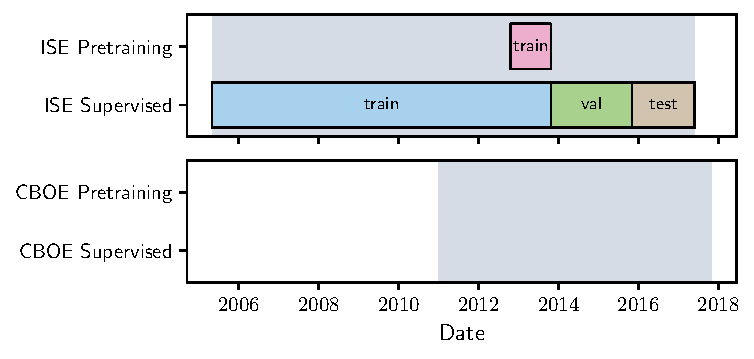
\includegraphics{train-test-split.pdf}
    \caption[Training Scheme on \glsentryshort{ISE} and \glsentryshort{CBOE} Sample]{Training scheme on \gls{ISE} and \gls{CBOE} sample. The train and validation set are split by time. Shaded area \mysquare{viz-gray} indicates the duration for which the dataset is available.}
    \label{fig:train-test-split}
\end{figure}

Overall, we use \gls{ISE} data from 2 May 2005 to 24 October 2013 to train and data between 25 October 2013 and 5 November 2015 to validate our models. The most recent trades until 31 May 2017 to assess the generalisation error.

Models are pre-trained on unlabelled samples from the last year of the training period. Given the significantly larger number of unlabelled customer trades, the pre-training period is reduced to one year to facilitate training on the available computing resources. Within the period, we filter out trades for which true label can be inferred, to avoid overlaps with the supervised training set. This is essential for self-training, as labelled and unlabelled data are provided to the model simultaneously.

\todo{Even quotes might be identical. Found this Fifth, options exchanges quote the same price most of the time because of the large tick size. For example, SEC (2007) shows that at least three exchanges quote the same NBBO price more than 75\% of the time. in \autocite{muravyevOrderFlowExpected2016}. Source is \autocite{securitiesandexchangecommissionReportConcerningExaminations2007}.}
We use the \gls{CBOE} sample past 5 November 2015 as a second test set, as visualised in \cref{fig:train-test-split}. Our evaluation approach is the most rigorous as it disallows any form of adaptation of the models, thereby ensuring a rigorous evaluation. Unlike transfer learning techniques such as parameter or model transfer, which expectedly improve model performance, we choose to forgo these techniques and demonstrate the effectiveness of our models without any transfer of knowledge. The start date ensures that leakage from the \gls{ISE} set is minimised. \footnote{The datasets contain features, such as the \gls{NBBO}, that are identical for both sets, assuming trades were executed at both exchanges simultaneously. Utilising the full \gls{CBOE} sample could result in exaggerated performance estimates the corresponding \gls{ISE} trade is used in training.}

Our train-test-split assumes that all subsets are drawn from the same distribution, so fitting a classifier on the training set and optimising for the validation set provides good estimates for the test set. To validate this assumption, we use adversarial validation. Specifically, we re-label all training samples with $y=-1$ and all trades of the validation set with $y=1$, train a classifier on a random subset of the composed dataset and predict class conformance. The performance is estimated using the \gls{MCC} of \textcite[][445]{matthewsComparisonPredictedObserved1975}, which ranges between $\left[-1, 1\right]$ and is insensitive to class imbalances.\footnote{Classes are imbalanced, due to the training set being three times the size of the validation set.} Assuming train and validation samples are sampled from the same distribution, the performance estimate is near a random guess, or $\operatorname{MCC} = 0$. For the mid-sized feature set, the \gls{MCC} is \num{0.364260805498287} suggesting training and validation sets are approximately similar. The next section discusses techniques used in training the classifiers.